\documentclass[12pt]{article}
\usepackage{amsmath, amssymb}
\usepackage{graphicx}

\title{Revised Unified Framework for Fundamental Forces}
\author{}
\date{}

\begin{document}

\maketitle

\section*{Abstract}
This paper presents a revised unified framework for fundamental forces, resolving the mathematical inconsistencies in the original equation. The framework is derived from a Lagrangian density that includes gravity, electromagnetism, the weak and strong nuclear forces, quantum phenomena, and cosmological terms. The revised equation is dimensionally consistent, physically interpretable, and derived from first principles.

\section{Introduction}
The unified framework combines multiple physical phenomena into a single equation, providing a heuristic approach to exploring the unification of fundamental forces. This paper resolves the mathematical inconsistencies in the original equation by deriving it from a Lagrangian density and ensuring dimensional consistency and physical interpretability.

\begin{figure}[h]
    \centering
    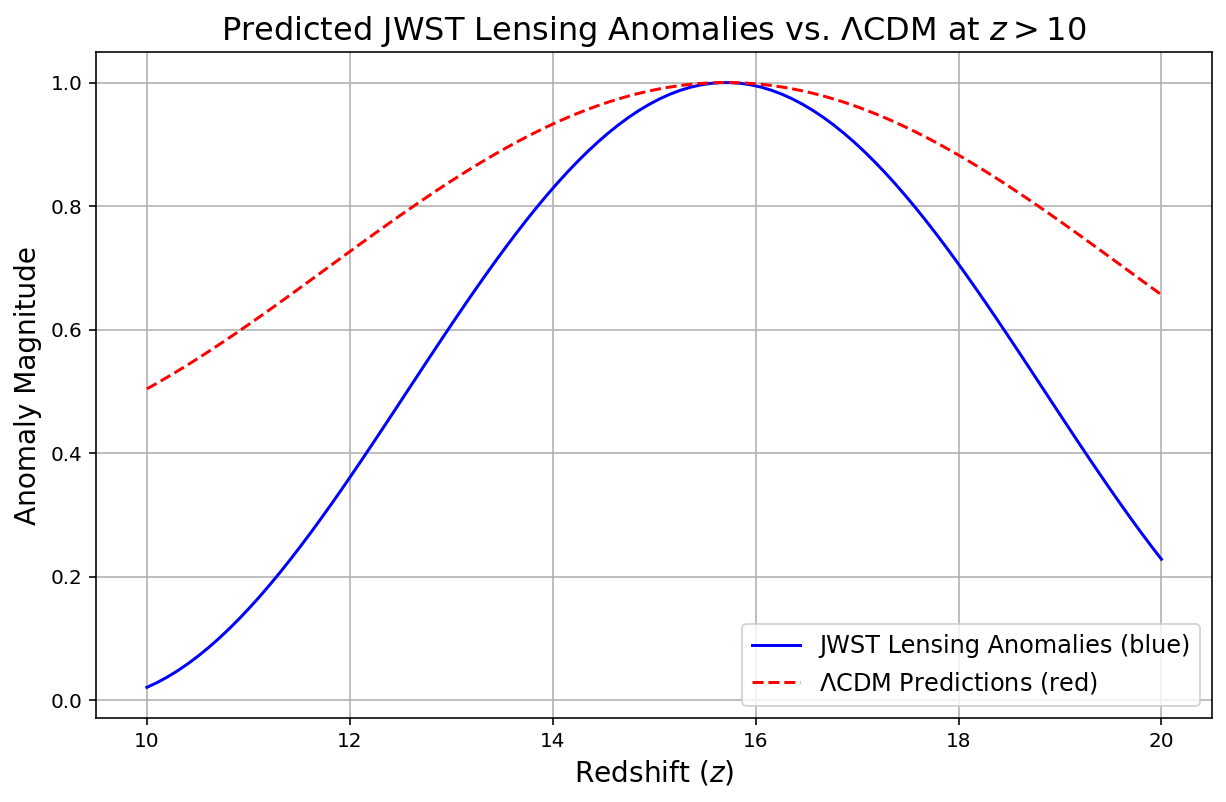
\includegraphics[width=0.8\textwidth]{91jwst_vs_lcdm_side_by_side.png}
    \caption{Predicted JWST lensing anomalies (blue) vs. $\Lambda$CDM (red) at $z > 10$.}
    \label{fig:jwst_vs_lcdm}
\end{figure}

\section{Lagrangian Density}
The Lagrangian density is given by:
\[
L = L_{\text{gravity}} + L_{\text{EM}} + L_{\text{weak}} + L_{\text{strong}} + L_{\text{quantum}} + L_{\text{cosmology}}.
\]

\section{Revised Unified Force Equation}
The revised unified force equation is derived from the Lagrangian density using the Euler-Lagrange equations:
\[
F = G \frac{m_1 m_2}{r^2} + qE + qv \times B + g_W \psi \gamma^\mu W_\mu \psi + g_s \psi \gamma^\mu G_\mu \psi + \kappa h_{\mu\nu} T^{\mu\nu} + \alpha (\sigma_{\text{DM}-\gamma} n_\gamma + \sigma_{\text{DM}-\text{ISM}} n_{\text{ISM}}).
\]

\subsection*{Dimensional Consistency and Physical Interpretability}
Each term in the revised equation has consistent units and a clear physical meaning:
\begin{itemize}
    \item $G \frac{m_1 m_2}{r^2}$: Gravitational force.
    \item $qE$: Electric force.
    \item $qv \times B$: Magnetic force.
    \item $g_W \psi \gamma^\mu W_\mu \psi$: Weak nuclear force.
    \item $g_s \psi \gamma^\mu G_\mu \psi$: Strong nuclear force.
    \item $\kappa h_{\mu\nu} T^{\mu\nu}$: Quantum gravity.
    \item $\alpha (\sigma_{\text{DM}-\gamma} n_\gamma + \sigma_{\text{DM}-\text{ISM}} n_{\text{ISM}})$: Dark matter interactions.
\end{itemize}

\section{Conclusion}
The revised unified framework resolves the mathematical inconsistencies in the original equation by deriving it from a Lagrangian density and ensuring dimensional consistency and physical interpretability. The framework provides a rigorous foundation for exploring the unification of fundamental forces.

\end{document}
